\documentclass[11pt,a4paper]{article}
\usepackage[utf8]{inputenc}
%\usepackage{ucs}
\usepackage{amsmath}
\usepackage{amsfonts}
\usepackage{amssymb}
\usepackage{parskip}
\usepackage{fullpage}
\usepackage{url}
\usepackage{algorithm}
\usepackage{algorithmic}
\usepackage{graphicx}
\usepackage{float}
\usepackage{subfigure}
\usepackage{fancyhdr}
\setlength{\headheight}{17.0pt}
\setlength{\headsep}{5.0pt}
\pagestyle{fancy}

\fancyhf{}
 
\setlength{\headsep}{16pt}
\setlength{\headheight}{19pt}
\lhead{\sf \scriptsize V. Hallberg, A. Hjalmarsson, J. Puigcerver, \\C. Rydberg and J. Stjernberg}
\chead{\sf \scriptsize Information Retrieval: \\ TweetRank - PageRank for Twitter}
\rhead{\sf \scriptsize DD2476  \\ \today}
\cfoot{\large \thepage}

\renewcommand{\algorithmicrequire}{\textbf{Input:}}
\renewcommand{\algorithmicensure}{\textbf{Output:}}

\author{V. Hallberg, A. Hjalmarsson, J. Puigcerver, \\C. Rydberg and J. Stjernberg\\
\footnotesize{\{victorha,alehja,joanpip,chrryd,stjer\}@kth.se}}
\title{\Huge TweetRank \\ \LARGE An adaptation of the PageRank algorithm to Twitter world}

\begin{document}
\maketitle
 \vspace{30px}
\begin{abstract}
\noindent
PageRank is an algorithm presented by Larry Page and Sergey Brin that allows to estimate the importance of a web page using the hyperlinks among them. This algorithm was originally the core of Google's search engine and proved to work very well in the web structure. Our task was to adapt the PageRank to work in the world of Twitter, instead of the web. This document presents the mathematical basis to compute, what we called, the \emph{TweetRank}, an algorithm to compute an approximation to \emph{TweetRank} based on Monte Carlo methods, and a simple search engine designed as a demonstration of our work.
\end{abstract}
%\\ \\ \\

\newpage

\tableofcontents  

\newpage

\section{Introduction}
Page and Brin defined the importance of a web page as the probability that at a certain time \cite{pagebmw98}, a person that randomly clicks on links will be visiting that web page. This assumption, called \emph{random surfing}, works really well on the World Wide Web since the navigation is driven by hyperlinks among web pages. 

Formally, the PageRank is the largest real eigenvector of the matrix $G$ defined as it follows:
\begin{equation}\label{eq:basic_pr}
G = \alpha R + (1-\alpha) L
\end{equation}

Each element $G_{i,j}$ represents the probability of visiting the web page $j$ given that the user is in the web page $i$. $G_{i,j}$ is defined as the weighted summation of $L_{i,j}$ and $R_{i,j}$.

$L_{i,j}$ represents the probability of visiting the web page $j$ following one of the links of the web page $i$, and $R_{i,j}$ represents the probability of randomly visiting the web page $j$ from web page $i$. $R_{i,j}$ is usually set to $\frac{1}{|W|}$ and it represents the probability of accessing the web page $j$ by a random access. 

In the world of Twitter, considering only direct references or hyperlinks among tweets it is not enough powerful to describe the importance of a Tweet, because the connectivity in Twitter is sparser than the Web. Some authors realised about this problem and presented alternatives to PageRank for ranking tweets in \cite{Duan:2010:ESL:1873781.1873815,DBLP:conf/webi/NagmotiTC10}. Other authors \cite{Duan:2010:ESL:1873781.1873815,Kwak:2010:TSN:1772690.1772751,DBLP:conf/wsdm/WelchSHC11} have described how to use PageRank to rank users based on the followers, the replies, etc. None of them have proposed a pure PageRank-based algorithm to rank tweets. S. Ravikumar et al. presented in \cite{DBLP:journals/corr/abs-1204-0156} an approach that first computes the PageRank for users, and then distributes it among tweets. This is similar to what we do to avoid the sparsity of Twitter, however our approach embeds this into the PageRank computation itself and not as a separate step.

In the next section, we present some basic concepts about Twitter that will be used to define the TweetRank.
\section{Twitter concepts}
Twitter\footnote{\url{http://www.twitter.com}} is a social network that allows users to send and read short messages called \emph{tweets}. There are many ways of interaction in Twitter: users can \emph{follow} other users and are notified about the posts from these \emph{followed} users, users can \emph{mention} other users on their tweets, they can re-post a tweet from an other user (\emph{retweet}) or they can \emph{reply} to a certain tweet. Additionally, a tweet can mention several \emph{hashtags}, which are usually used to designate the topic that the tweet is talking about (for instance: \emph{\#politics}, \emph{\#Twitter} or \emph{\#ChampionsLeague}). Given that concepts\footnote{\url{http://support.twitter.com/entries/13920-frequently-asked-questions}}, we define the following matrices representing the different relationships. \\

The matrix $RT$ describes the \emph{retweet} relationship among different tweets. 
\begin{equation}\label{eq:retweet_rel}
RT_{i,j} = \begin{cases}
1 & \text{if tweet } i \text{ retweets } j \\
0 & \text{otherwise}
\end{cases}
\end{equation}

Notice that $RT$ is a $|T| \times |T|$ matrix ($T$ is the set of tweets), where each row has at most one non-zero element (since a tweet $i$ can only retweet a single tweet $j$) and the relationship is asymmetric (if a tweet $i$ retweets $j$, then $j$ does not retweet $i$). \\

The matrix $RP$ describes the \emph{reply} relationship among different tweets, with the same properties of $RT$.
\begin{equation}\label{eq:reply_rel}
RP_{i,j} = \begin{cases}
1 & \text{if tweet } i \text{ replies } j \\
0 & \text{otherwise}
\end{cases}
\end{equation}

The matrix $MN$ describes the \emph{mention} relationship among tweets and users. $MN$ is a $|T| \times |U|$, where $U$ is the set of users. 
\begin{equation}\label{eq:mention_rel}
MN_{i,j} = \begin{cases}
1 & \text{if tweet } i \text{ mentions user } j \\
0 & \text{otherwise}
\end{cases}
\end{equation}
Notice that $m_i = \sum_{j \in U} MN_{i,j}$ is the number of mentions in the tweet $i$. \\

The matrix $FW$ describes the \emph{following} relationship among users. $FW$ is a $|U| \times |U|$ matrix.
\begin{equation}\label{eq:following_rel}
FW_{i,j} = \begin{cases}
1 & \text{if user } i \text{ follows user } j \\
0 & \text{otherwise}
\end{cases}
\end{equation}
Notice that $f_i = \sum_{j \in U} FW_{i,j}$ is the number of users followed (\emph{friends}) by user $i$. \\

The matrix $HT$ describes the relationship among tweets and hashtags. $FW$ is a $|T| \times |HS|$ matrix, where $HS$ is the set of hashtags.
\begin{equation}\label{eq:hashtags_rel}
HT_{i,j} = \begin{cases}
1 & \text{if tweet } i \text{ includes hashtag } j \\
0 & \text{otherwise}
\end{cases}
\end{equation}
Notice that $th_i = \sum_{j \in HS} HT_{i,j}$ is the number of hashtags included in tweet $i$ (row sum). Similarly, $ht_j = \sum_{i \in |T|} HT_{i,j}$ is the number of tweets that used the hashtag $j$ (column sum).
\section{TweetRank definition}\label{sec:tweetrank_definition}
TweetRank also defines the relevance of a tweet as the largest real eigenvector of a matrix $G'$, as PageRank did. However, our matrix will take into account not only the direct relationships among tweets (retweets and replies). The idea is that tweet $j$ can be accessed from tweet $i$ by:  
\begin{itemize}
\item $R_{i,j} = \frac{1}{|T|}$, random access probability.
\item $L_{i,j}$, probability of accessing tweet $j$ following a retweet or reply on tweet $i$.
\item $M_{i,j}$, probability of accessing tweet $j$ following a mention on tweet $i$.
\item $F_{i,j}$, probability of accessing tweet $j$ accessing the owner of tweet $j$ from the friends of $i$'s owner, and then randomly choosing $j$.
\item $H_{i,j}$, probability of accessing tweet $j$ accessing a hashtag used by $j$ from the hashtags used by $i$, and accessing randomly choosing $i$.
\end{itemize}

Given that, elements in $G'$ are defined as (with $\alpha + \beta + \gamma + \delta + \epsilon = 1$):
\begin{equation}\label{eq:tweetrank}
G'_{i,j} = \alpha R_{i,j} + \beta L_{i,j} + \gamma M_{i,j} + \delta F_{i,j} + \epsilon H_{i,j}
\end{equation}

\subsubsection*{$L_{i,j}$ approximation}
\begin{equation}\label{eq:ref_prob}
L_{i,j} = RT_{i,j} + RP_{i,j}
\end{equation}

The previous equation uses the result of equations \ref{eq:retweet_rel} and \ref{eq:reply_rel}. Note that a tweet can be either a retweet, a reply or none of them (new post). So, $RT_{i,j} + RP_{i,j}$ is equal to 0 or 1, and there are at most one non-zero element in the $i$-th row of matrix $L$.

\subsubsection*{$M_{i,j}$ approximation}
First, probability of visiting the profile of a user $j$ from a mention in a tweet $i$ is defined as $FM_{i,j}$. Remember that $m_i$ was defined as the number of mentions in tweet $i$. This definition uses the result of equation \ref{eq:mention_rel}. Then $M_{i,j}$ is defined in \ref{eq:mentions_probability}.

\begin{equation}
FM_{i,j} = \begin{cases}
\frac{MN_{i,j}}{m_i} & \text{if } m_i > 0 \\
0 & \text{otherwise}
\end{cases}
\end{equation}

\begin{equation}\label{eq:mentions_probability}
M_{i,j} = \frac{FM_{i, u_j}}{ |t \in T : u_t = u_j|}
\end{equation}
Note that $|t \in T : u_t = u_j|$ is just the number of tweets from user $u_j$.

\subsubsection*{$F_{i,j}$ approximation}
In the first place, probability of visiting the profile of user $j$ accessing the following list of user $i$ is defined as $FF_{i,j}$. Notice that $f_i$ is the number of users followed by user $i$. Using this probability, $F_{i,j}$ is defined in \ref{eq:follows_probability}.
\begin{equation}
FF_{i,j} = \begin{cases}
\frac{FW{i,j}}{f_i} & \text{if } f_i > 0 \\
0 & \text{otherwise}
\end{cases}
\end{equation}

\begin{equation}\label{eq:follows_probability}
F_{i,j} = \frac{FF_{u_i, u_j}}{ |t \in T : u_t = u_j|}
\end{equation}
Note that $|t \in T : u_t = u_j|$ is just the number of tweets of user $u_j$.

\subsubsection*{$H_{i,j}$ approximation}
First, let's define the probability that a tweet $j$ is visited from tweet $i$, using the hashtag $k$. Remember that $ht_k$ denotes the number of tweets that use the hashtag $k$ and $th_i$ denotes the number of hashtags that are included in tweet $i$.

\begin{equation}
HP_{i,j,k} = \begin{cases}
\left( \frac{ HT_{j,k} }{ ht_k } \right) \cdot \left( \frac{ HT_{i,k} }{ th_i } \right) & \text{if } ht_k > 0 \wedge th_i > 0 \\
0 & \text{otherwise}
\end{cases}
\end{equation}

Note that $HP_{i,j,k}$ will be greater than zero if, and only if, both $i$ and $j$ included the hashtag $k$. 

Then, $H_{i,j}$ is defined as:
\begin{equation}
H_{i,j} = \sum_{k \in HS} HP_{i,j,k}
\end{equation}

\subsection{Weighting using \emph{hashtags}}
An extension of the previous definition of $G'$ could take into account some measure of similarity between users. Our idea is that users that share common interests would rank higher tweets from users with similar interests. We propose to use the \emph{hashtag} concept on Twitter to measure what a user talks about. However, as we will discuss later, the assumption behind this approach might be not true in many cases as we will discuss later.

\subsubsection*{Hashtag similarity}
The matrix $HT'$ represents the relation among users and hashtags, that is, wich hashtags are used (and how many times) by each user. $HT'$ is defined as it follows.
\begin{equation}
HT'_{i,j} = \text{Number of times that user } i \text{ uses the hashtag } j
\end{equation}

Each row $i$ in the matrix $HT'$ represents a feature vector $\vec{h}_i$ of the user $i$. The similarity between two users $i$ and $j$ is defined as the cosine of the angle formed by the vectors $\vec{h}_i$ and $\vec{h}_j$.
\begin{equation}
d_{i,j} = \frac{\vec{h}_i \cdot \vec{h}_j}{ |\vec{h}_i| \cdot |\vec{h}_j|}
\end{equation}

\subsubsection*{$G'$ extension to $G''$}
Given $Z = \beta' L + \gamma' M + \delta' F + \epsilon' H$ (being $\beta' = \frac{\beta}{1-\alpha}$, $\gamma' = \frac{\gamma}{1-\alpha}$, $\delta' = \frac{\delta}{1-\alpha}, \epsilon' = \frac{\epsilon}{1 - \alpha}$),  $G'$ can be expressed as:
\begin{equation}
G' = \alpha R + \beta L + \gamma M + \delta F + \epsilon H =  \alpha R + (1-\alpha) Z
\end{equation}

Given that, we extended the definition of $G'$ and $Z$ to take into account the similarity between two users defined before. 
\begin{equation}
Z'_{i,j} = \frac{d_{u_i,u_j} Z_{i,j}}{\sum_{j \in T}{d_{u_i,u_j} Z_{i,j}}}
\end{equation}

Note that this definition presents a little problem with users that have orthogonal feature vectors or zero-vectors: the distance between them will be 0, and the $Z'_{i,j}$ element will be 0 as well. A constant value $k > 0$ to $d_{u_i,u_j}$ is added to ensure that as long as $Z_{i,j}$ is different to 0, $Z''_{i,j}$ will be different to zero as well.
\begin{equation}
Z''_{i,j} = \frac{ (d_{u_i,u_j} + k) Z_{i,j}}{\sum_{j \in T}{(d_{u_i,u_j} + k) Z_{i,j}}}
\end{equation}

Thus, the weighted-probability of visiting the tweet $j$ from tweet $i$ would be expressed by the matrix $G''$ defined as:
\begin{equation}
G'' = \alpha R + (1 - \alpha) Z''
\end{equation}

\subsubsection*{Disadvantages of similarity weighting}
This extension presents some disadvantages. The first one is that adding a new parameter $k$ adds more complexity to our system and makes it harder to select the optimal values for the model parameters. Choosing a too high value for $k$ would take away the effect of the weighting and choosing a value that is too small would make the already sparse graph matrix of Twitter even sparser.

The second problem is given by the assumption which this approach relies on: the fact that users would rank higher tweets from other users with similar interests. For example, suppose we have two users that use to post comments about politics: it seems unlikely that a conservative person would give a high score to tweets from progressive users. Even if they share the same hashtag, the opinion expressed in both tweets may be very different.

Because of these two reasons we did not implement this extension in our TweetRank computation. However, note that an adaptation of algorithm \ref{algo:alg1} can be easily implemented to take into account that score. The only thing that has to be changed is how the visit counter is updated.

\section {Implementation}

\subsection{Overview}
We implemented a small search engine that uses TweetRank to rank the tweets crawled from Twitter. The search engine has three main components: the crawler module, the \emph{ranker} module, and the Solr module. Figure \ref{fig:overview} represents the communication among the different components.

\begin{figure}
\centering
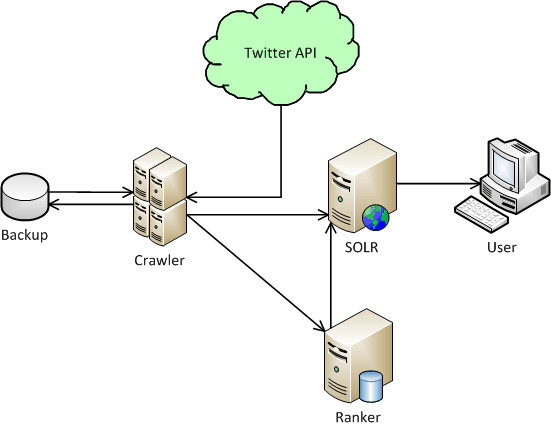
\includegraphics[width=0.4\textwidth]{../tweetmap.png} 
\caption{Overview of our search engine.}
\label{fig:overview}
\end{figure}

The crawler continuously fetches tweets from Twitter users using the Twitter API, saves the data to disk as a backup, parses it to extract the required information for our algorithms, and sends the parsed data to the ranker and the Solr module. The crawler sends the data to Solr using XML its XML POST request specification and it sends data to the ranker using a protocol designed by us. The crawler was designed to run in multiple threads or multiple machines.


\subsection{TweetRank}\label{sec:tweetrank_implementation}
Algorithm \ref{algo:alg1} is used to compute the TweetRank score and it is an adaptation of the classic Monte Carlo complete path stopping at dangling nodes method. The graph from Twitter $G$ is just the set of relationships described in section \ref{sec:tweetrank_definition}. Algorith \ref{algo:alg1} includes some predefined functions that are not described here, however we thought that their name is descriptive enough.

\begin{algorithm}
\caption{Compute TweetRank using MC complete path stopping at dangling nodes}
\label{algo:alg1}
{\fontsize{8}{8}\selectfont
\begin{algorithmic}
\REQUIRE Probabilities $\alpha, \beta, \gamma, \delta, \epsilon$ such that $\alpha+\beta+\gamma+\delta+\epsilon=1$, Twitter graph $G$ and $M \in \mathbb{N}$ such that $T\times M \in O(T^2)$.
\ENSURE $\pi$, TweetRank of tweets in $T(G)$.
\STATE $V_t \leftarrow 0, \forall t \in T$ \COMMENT{Visit counter for tweets}
\STATE $CP_0 \leftarrow \alpha$ \COMMENT{Cumulative probabilities for each action}
\FORALL{$t \in T(G)$}
\FOR {$m=1$ to $M$}
\STATE $ct \leftarrow t$
\STATE $stop \leftarrow False$
\WHILE {$\neg stop$}

\STATE $CP_1 \leftarrow CP_0 + \beta \cdot hasRetweetOrReply(ct)$
\STATE $CP_2 \leftarrow CP_1 + \gamma \cdot hasMentions(ct)$
\STATE $CP_3 \leftarrow CP_2 + \delta \cdot hasFriends(user(ct))$
\STATE $CP_4 \leftarrow CP_3 + \epsilon \cdot hasHashtags(ct)$

\STATE $r \leftarrow UniformRandomNumber(0, CP_4)$ \COMMENT{This ensures that all rows sums 1.0}

\IF { $r \leq CP_0$ }
\STATE $ct \leftarrow jumpToRandomTweet()$
\STATE $stop \leftarrow True$
\ELSIF { $r \leq CP_1$ }
\STATE $ct \leftarrow jumpToRetweetOrReply(ct)$
\ELSIF { $r \leq CP_2$ }
\STATE $ct \leftarrow jumpToMentionTweet(ct)$
\ELSIF { $r \leq CP_3$ }
\STATE $ct \leftarrow jumpToFriendTweet(ct)$
\ELSE
\STATE $ct \leftarrow jumpToHashtagTweet(ct)$
\ENDIF
\STATE $V_{ct} \leftarrow V_{ct} + 1$ 
\ENDWHILE
\ENDFOR
\ENDFOR
\STATE $\pi_t \leftarrow Normalize(V)$ \COMMENT{TweetRank as the normalized visit vector}
\end{algorithmic}}
\end{algorithm}

Observe that the running time of algorithm \ref{algo:alg1} is non-deterministic, since it depends on the structure of the graph itself and the $\alpha$ parameter. Assuming random access memory, and no dangling nodes in graph, the previous algorithm has an expected running time bounded by $O(|T| \times M \times \mathbb{E}[|w|])$, where $\mathbb{E}[|w|]$ is the expected length of the random walk. The expected length of the random walk is obtained from the following
equation:
\begin{equation}
\mathbb{E}[|w|] = \sum_{k=1}^{\infty} P(|w| = k) \cdot k = \sum_{k=1}^{\infty} (1 - \alpha)^{k-1} \cdot \alpha \cdot k = \frac{1}{\alpha}
\end{equation}

Given that $|T| \times M$ must be $O(|T|^ 2)$ to ensure a good approximation of TweetRank, the expected running time of algorithm \ref{algo:alg1} is:
\begin{equation}\label{eq:running_time}
O(|T| \times M \times \mathbb{E}[|w|]) = O(|T|^2 \times \frac{1}{\alpha}) = O(|T|^2)
\end{equation}

Note that equation \ref{eq:running_time} is an upper bound on the expected running time if the graph contains dangling nodes. On the other side, the assumption of random access memory might be a problem for a large index which does not fit in the main memory of a single machine. However, implementing TweetRank on a large-scale distributed system is not the approach of this work and we will made this assumption to keep the analysis simple.
%\subsection{HTTP server}

The Python crawler sends data using the POST request method in the HTTP protocol to the Java program which contains a HTTP server. For this to work, we have developed a simple protocol which these programs use to communicate. The protocol looks like this:

\begin{itemize}
	\item \textbf{Type} - The type of the data being sent.
	\begin{itemize}
		\item \textbf{RT} or \textbf{RP} - This tweet is a reply/retweet of the referenced tweet.
		\item \textbf{FW} - List of users that this user follows.
		\item \textbf{HT} - List of hashtags mentioned in this tweet.
		\item \textbf{MN} - List of users mentioned in this tweet.
		\item \textbf{TW} - List of tweets written by this user.
	\end{itemize}
	\item \textbf{ID} The ID of this user/tweet. (User for FW \& TW, tweet for all others.)
	\item \textbf{refID} Depends on the type.
	\begin{itemize}
		\item[] (RT/RP): Referenced tweet ID. Multiple IDs not allowed.
		\item[] (FW): User ID(s) that this user follows.
		\item[] (HT): Hashtag(s) mentioned in this tweet.
		\item[] (MN): User ID(s) of users that are mentioned in this tweet.
		\item[] (TW): Tweet ID(s) of tweets that are written by this user.
	\end{itemize}
\end{itemize}

\textit{Implementation note: all IDs are handled as numbers of type Long. refID for HT/Hashtag and the type parameter are handled as Strings.}

Upon successful parsing in the HTTP server, the data is sent to the ranker which adds it to the lists of already existing data. % Too extensive, I wouldn't talk about the crawler and the http server too much, just mention them in the overview.


\subsection{Solr - Incomplete!}
Solr 3.6 were used as the query interface for the TweetRank. It receives the Tweets from the Crawler by XML POST requests and indexes them. To improve the usability we also make use of the built-in tf-idf scoring that is offered by Solr/Lucene.

The TweetRank scores which are calculated at the ranker component which then prints the results as key value pairs in a plain text formatted file. This file is then used by Solr as an ''External file field'' which we combine with the other ranking attributes. The ranking attributes that we base our weighting on are the following:

\begin{itemize}
	\item \textbf{Hashtag} - If a hashtag $H$ is mentioned in the tweet $T$ and found in the query $Q$, we give additional score to $T$ for the query $Q$.
	\item \textbf{Username} - If the username of the author of tweet $T$ is found in query $Q$, we give additional score to $T$ for the query $Q$.
\end{itemize}

In addition to the the mentions above, we give an additional score to tweets that have been tweeted recently. The function we used for this additional date score is following: 

\begin{equation}
\frac{a}{m*x+b}
\end{equation}

where we have defined $x$ as the age of the tweet in milliseconds, $m = 3.16E^{-11}$, $a = 0.08$ and $b = 0.05$. 
\section{Experiments}
Measuring the quality of the TweetRank score is difficult because there are no reference corpora to be tested on, the only thing that we did was to try it together with Solr and checked that the results quality was good.

We implemented the Power Iteration method for TweetRank and computed the TweetRank for small sets of tweets with a precision of $10^{-10}$. Table \ref{table:mc_errors} shows the relative error between the ranking obtained by Power Iteration and our Monte Carlo approximation. We also plotted the sorted list of TweetRank values in log-log scale and checked that it follows closely the power law, as it was stated by \cite{Avrachenkov:2007:MCM:1272804.1272825}. Figure \ref{fig:tweetrank_powerlaw} shows this fact.

\begin{table}
\centering
\begin{tabular}{|c|c|}
\hline Tweets & Relative error (\%) \\
\hline 5658 & $8.13109904923 \cdot 10^{-4}$ \\
\hline 17174 & $6.10684768151 \cdot 10^{-5}$ \\
\hline 32828 & $7.79007058261 \cdot 10^{-5}$ \\
\hline 46934 & $2.724550120103 \cdot 10^{-5}$ \\
\hline
\end{tabular}
\caption{Relative error between our algorithm and Power Iteration with $10^{-10}$ precision}
\label{table:mc_errors}
\end{table}

\begin{figure}
\centering
\subfigure[Sorted TweetRank, loglog scale]{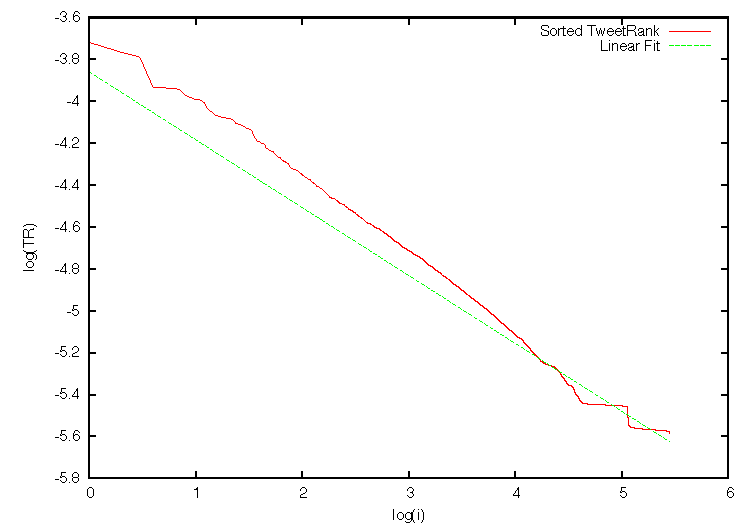
\includegraphics[width=0.4\textwidth]{tweetrank_powerlaw.pdf}\label{fig:tweetrank_powerlaw}}
\qquad
\subfigure[Running time vs. tweets]{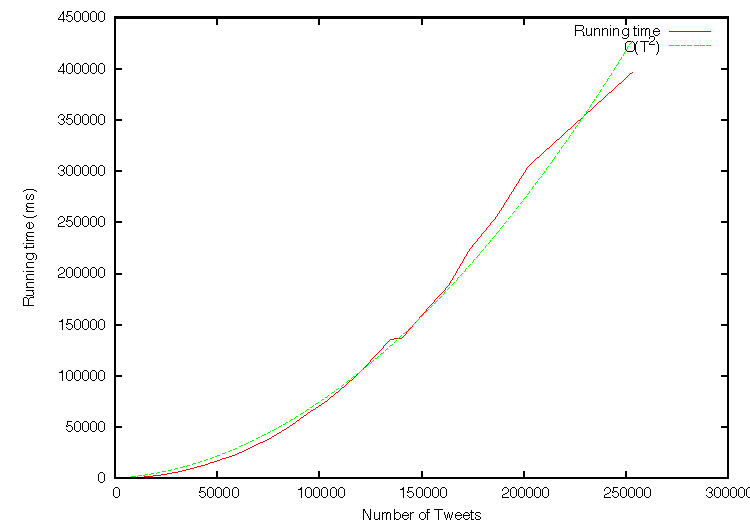
\includegraphics[width=0.4\textwidth]{tweetrank_times.pdf}\label{fig:tweetrank_times}} 
\caption{Experiment results}
\end{figure}

Figure \ref{fig:tweetrank_times} shows the number of tweets versus the running time. We see that a quadratic curve fits very well with the experimental data, which confirms our analysis of the expected running time described in equation \ref{eq:running_time} (section \ref{sec:tweetrank_implementation}). These results were obtained on a machine and parameters specified in table \ref{table:machine_spec}. 

\begin{table}
\centering
\begin{tabular}{|c|c|}
\hline Processor & Intel Core i5, 2 cores at 2.4GHz, 64 bits \\
\hline Memory & Main: 4GB DDR3, Cache L3: 3MB, Cache L2: 256KB \\
\hline OS &  Mac OS X 10.6.8 Snow Leopard \\
\hline Compiler & javac 1.6.0\_31, 64 bits, no optimization parameters \\
\hline Others & 8 threads, $\alpha = 0.2, \beta = 0.4, \gamma = 0.2, \delta = 0.04, \epsilon = 0.16, M = T/100$ \\
\hline
\end{tabular}
\caption{Specification of the machine used for experimentation}
\label{table:machine_spec}
\end{table}

It's important to observe that our model has many parameters to be adjusted. Design a good set of experiments to choose the best values would require a lot of time and also lot of time to be tested. For estimating the optimal values for the probabilities used by our algorithm, the simplest solution would be trying different combinations of their values and try to find the one that produces better results. However, this would require a tremendous amount of time and, even more important, would require a labelled dataset to measure the precision and recall of the search engine.

An other approach, would be monitor those probabilities on real users. For example, installing a plug-in on the web browser that registers the activity of the user (when the user clicks on a retweet or reply, on a mentioned user, on the friends list, etc). To preserve anonymity, this would be a plug-in installed in volunteer's browsers and the data collected would not contain any personal information (it is not important for us which tweet is viewing the user, but how he or she got to it). Using this data, one could estimate those probabilities and use the estimated value to compute the TweetRank.
\section{Conclusion}
We adapted the definition of PageRank to Twitter context where direct references among tweets (retweets or replies) are not the usual way to surf on Twitter. We proposed to take into account also mentions, followers and hashtags to determine the importance of a tweet. We presented an extension of the previous model which considers the similarity between users in terms of common hashtags. 

We have disscussed several during the previous sections the advantages and disadvantages of our model and the algorithm used to compute the TweetRank. However, the main disadvantage to our current implementation is that each time a new tweet is added, a new computation for the whole set of tweets is required. And this approach does not scale in a dynamic environment like Twitter where millions of tweets are published each second. Computing PageRank on a dynamic network is a well-studied problem. Our model could be adapted to the approaches described in \cite{Bahmani:2010:FIP:1929861.1929864,Desikan:2005:IPR:1062745.1062885} easily, but that is more over the purpose of this work.

\newpage

\bibliographystyle{abbrv}
\bibliography{bibliography}

\end{document}